\section{Physics}\label{sec:physics}

In this section we will be looking at some of the physics behind the equations we will be using in our models. We start by looking at the absorption and desorption of Metal Hydride Materials in Section~\ref{subsec:metal_hydrides}, and explain how we get to the absorption equations in our models. Then we will be looking at the flow of our Hydrogen gas in Section~\ref{subsec:flow_model}, as these will be the most important equations for our models.

\subsection{Absorption and Desorption in Metal Hydride Materials}\label{subsec:metal_hydrides}

Metal Hydrides have been researched extensively. They are materials that can absorb Hydrogen gas, and store it in a solid form. This is done by the metal hydride absorbing the hydrogen gas, and forming a chemical bond with it. This is a reversible process, and the hydrogen can be released from the metal hydride by heating it up. This makes metal hydrides a good candidate for hydrogen storage, as they can store large amounts of hydrogen in a small volume. The chemical reaction for the absorption and desorption of hydrogen in metal hydrides is surprisingly simple, and can be given by the following chemical reaction\cite{Sandrock1999}:
\begin{align*}
    \ce{M + \frac{x}{2} H2 &<=>[\ce{H2}] MH_x}
\end{align*}
Where $M$ is the metal, $H_2$ is the hydrogen gas, and $MH_x$ is the metal with Hydrogen attached to it. $x$ is the number of hydrogen atoms that can be absorbed by the metal. The absorption and desorption of hydrogen in metal hydrides is a reversible, but has a hysteresis effect, meaning that the absorption and desorption curves are not the same. A schematic of the absorption and desorption curves can be seen in Figure~\ref{fig:absorption_desorption}. From now on if we talk about absorption,  we will be looking at the upper part of the curve, and if we talk about desorption, we will be looking at the lower part of the curve. For these parts, the mass absorption, and desorption rates are given by\cite{Jemni1995}:
\begin{align}
    \dot m(\rho, \rho_s) &= C_a \exp(- \frac{E_a}{R \, T}) \,
    \log( \frac{p_p}{p_{eq,a}} ) \, (\rho_{sat} - \rho_s(t)) \, ,\\
    \dot m(\rho, \rho_s) &= C_d \exp(- \frac{E_d}{R \, T}) \,
    (1 - \frac{p_p}{p_{eq,d}}) \, (\rho_s(t) - \rho_o) \, ,
\end{align}
where $C_a$ and $C_d$ are the absorption and desorption rate constants, $E_a$ and $E_d$ are the activation energies for absorption and desorption, $R$ is the universal gas constant, $T$ is the temperature, $p_p$ is the pressure of the hydrogen gas, $p_{eq,a}$ and $p_{eq,d}$ are the equilibrium pressures for absorption and desorption, $\rho_{sat}$ is the saturation density of the metal hydride, $\rho_s(t)$ is the density of the metal hydride at time t, and $\rho_o$ is the initial density of the metal hydride.

In both papers they also calculate the equilibrium pressures for absorption and desorption using the Van't Hoff equation, which is given by:
\begin{equation}
    \log\left(\frac{p_{eq}}{P_{ref}}\right) = A-\frac{B}{T}
\end{equation}
Where $P_{ref}$ is the reference pressure set to $1MPa$, $A$ and $B$ are constants that depend on the metal hydride, set to $10.7$ and $3704.6$ for absorption, and $10.57$ and $3704.6$ for desorption.

\subsubsection*{Model Assumptions}

In our first model we assume constant temperature, and pressure, and we will simplify the absorption and desorption rates accordingly. The gas is however not pure hydrogen, and $\rho_g$ will be the ratio of hydrogen in the gas mixture. The absorption and desorption rates will then be given by:

\begin{equation}\label{eq:phy_dotm_model1}
    \begin{aligned}
        \dot m(\rho_g, \rho_s) &= A_a^1 (\rho_{sat} - \rho_s(t)) \, \rho_g  \\
        \dot m(\rho_g, \rho_s) &= A_d^1 (\rho_s(t) - \rho_o) \, \rho_g 
    \end{aligned}
\end{equation}
where $A_a^1$ and $A_d^1$ are constants that depend on the temperature, pressure, and the properties of the metal hydride. In our more advanced models we will be modelling pressure and assume that the temperature is constant. Now $\rho_g$ is not a ratio of H2 gas in the mixture but the density of the purely H2 gas. We will then have the following absorption and desorption rates:
\begin{equation}\label{eq:dotm_model_4}
    \begin{aligned}
        \dot m(\rho_g, \rho_s) &= A_a^2 \log \left( \frac{RT\rho_g}{p_{eq,a}} \right)(\rho_{sat} - \rho_s(t))  \\
        \dot m(\rho_g, \rho_s) &= A_d^2 \left( 1 - \frac{RT\rho_g}{p_{eq,d}} \right)( \rho_s(t) - \rho_o) \, ,
    \end{aligned}
\end{equation}
where $A_a^2$ and $A_d^2$ are constants that depend on the temperature, and the properties of the metal hydride. We also assumed the ideal gas law to relate the pressure and density of the hydrogen gas.


\begin{figure}
    \centering
    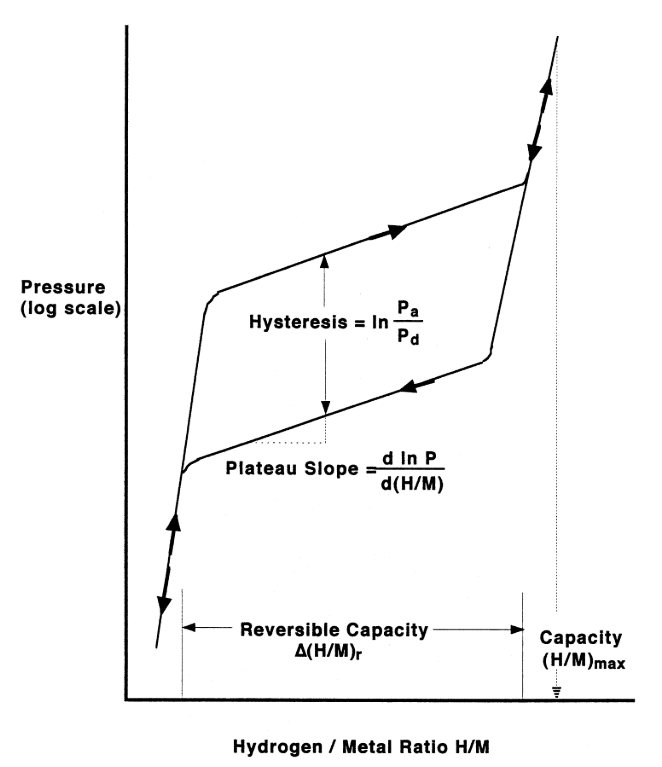
\includegraphics[width=0.4\textwidth]{figures/phy_hysteresis_curve.png}
    \caption{Schematic of the absorption and desorption curves of metal hydrides. The x-axis is the ratio between Hydrogen and Metal, and the capacity can therefor be interpreted as a measure for $x$ in $MH_x$. The absorption curve is the left and upper lines, the desorption is given in the right and lower lines. The hysteresis effect can be seen in the difference between the two curves. Schematic from Sandrock et al.\cite{Sandrock1999}}
    \label{fig:absorption_desorption}
\end{figure}


\subsection{Flow}\label{subsec:flow_model}
The governing equations consist of the conservation equations (mass, momentum and energy) together with constitutive equations describing the fluid properties. Assuming a Newtonian fluid, the constitutive relation for the stress tensor leads to the Navier–Stokes equations. The conservation equations are derived from the fundamental laws of physics, while the constitutive equations describe the material properties of the fluid. We will not be looking at the energy equation, as we assume constant temperature in our models. The conservation equations are given by (in their continuous form):

\begin{equation}\label{eq:continuity_equation}
    \partial_t \rho + \nabla \cdot (\rho \mathbf{u}) = \dot{m}
\end{equation}
Where $\rho$ is the density of the fluid, $\mathbf{u}$ is the velocity of the fluid, and $\dot{m}$ is the mass source term. The mass source term is given by the absorption and desorption rates we derived in Section~\ref{subsec:metal_hydrides}. The first term represents the local rate of change of mass, while the second term represents the net mass flux leaving the control volume. Together, they equal the volumetric mass source term due to absorption or desorption.

For Navier-Stokes, I like a little derivation starting from Newton's second law. Lets look at a small volume of fluid, now we get:

\begin{align*}
    \mathbf{F} &= m \, \mathbf{a} \\
    &= m \, \frac{D\mathbf{u}}{Dt} \\
    &= m \, (\partial_t \mathbf{u} + (\mathbf{u} \cdot \nabla) \mathbf{u}) \\
    \implies \frac{\mathbf{F}}{V} &= \rho \, (\partial_t \mathbf{u} + (\mathbf{u} \cdot \nabla) \mathbf{u})
\end{align*}
where $\mathbf{F}$ is the force, $m$ is the mass, $\mathbf{a}$ is the acceleration, $V$ is the volume, and $\rho$ is the density. Relevant forces acting on the fluid are the pressure gradient, the viscous forces, and we neglect any external forces (no gravity, no electromagnetic forces). These are given by:

\begin{align*}
    \frac{\mathbf{F}_{p}}{V} &= - \nabla p \\
    \frac{\mathbf{F}_{v}}{V} &= \mu \Delta \mathbf{u} \\
    % \frac{\mathbf{F}_{e}}{V} &= \mathbf{f}
\end{align*}
Where $p$ is the pressure, $\mu$ is the dynamic viscosity, and $\mathbf{f}$ is the external force. For the viscosity, we did assume a Newtonian fluid. Combining above equations, we get the Navier-Stokes equation:

\begin{align}
    \rho \, (\partial_t \mathbf{u} + (\mathbf{u} \cdot \nabla) \mathbf{u}) &= - \nabla p + \mu \Delta \mathbf{u}
\end{align}

Stokes:
\begin{equation}\label{eq:stokes_equation}
    \nabla \cdot \sigma + \mathbf{f} = 0
\end{equation}


\subsubsection*{Model Assumptions}
For our first spacially coupled models, we aim to measure the density of hydrogen gas $\rho_g$ in the battery, and the saturation of the metal hydride $\rho_s$. We do not yet aim to measure velocity of the gas and it is assumed that the flow is constant through the battery. The density of the hydrogen gas is seen as a fraction of the total density of the gas mixture, and we will assume that the gas mixture is incompressible. Thus in essence: $\rho = \rho_g + \rho_{other}$, where $\rho_{other}$ is the density of the other gases in the mixture. Since this is assumed constant, we can neglect it in our models, and we only have to look at Diffusion and Convection of the hydrogen gas:

\begin{equation}
    \left\{ \begin{aligned}
        \partial_t \rho_g &= D \nabla^2 \rho_g -\mathbf{v}\partial_x\rho_g - \dot{m}(\rho_g, \rho_s) \\
        \partial_t \rho_s &= \dot{m}(\rho_g, \rho_s)
    \end{aligned} \right.
\end{equation}